\documentclass[11pt]{article}
\usepackage[margin=1in]{geometry} 
\usepackage{amsmath}
\usepackage{tcolorbox}
\usepackage{amssymb}
\usepackage{amsthm}
\usepackage{commath}
\usepackage{lastpage}
\usepackage{fancyhdr}
\usepackage{accents}
\usepackage{csquotes}
\usepackage{soul}
\newcommand{\ubar}[1]{\underaccent{\bar}{#1}}
\pagestyle{fancy}
\setlength{\headheight}{40pt}


\newenvironment{solution}
  {\renewcommand\qedsymbol{$\blacksquare$}
  \begin{proof}[Solution]}
  {\end{proof}}
\renewcommand\qedsymbol{$\blacksquare$} % add packages, settings, and declarations in settings.tex

\begin{document}

\lhead{Yida Liu} 
\rhead{EECS 416 Spring 2020 \\ Convex Optimization for Engineering \\ Homework 2} 
\cfoot{\thepage\ of \pageref{LastPage}}


\section{Circle from Rubber}

\textbf{Decision variables:} The center of the circle $C_i=(x_i, y_i)$, and the radius $r_i$, for $i \in [1, 2, 3]$

\textbf{Objective function:} The problem seeks to minimize the waste after cutting, which is equivalent to say the total shape of the circles are maximized. 
$$
\max \pi\sum_i r_i^2
$$

\textbf{Constraints:}
\begin{enumerate}
    \item Non-overlapping circles: circles cannot overlap, otherwise it would not be the shape of the circle when cut. The distance between the center of two circle must be larger than the sum of their radii. Therefore, for each combination of circle $i$ and $j$, we must have constraint
    $$
    (x_i - x_j)^2 + (y_i - y_j)^2 \geq (r_i + r_j)^2
    $$
    
    \item Circle within bound: circles must be enclosed by the polygon that the points formed. To formulate this, we consider that the distance from the circle center to each of the edges of the polygon must be greater than the radius of the circle. We know how to calculate the formula for lines given two points m and n:
    $$
    ax + by = c, a = (x_m - x_n), b = (x_n - x_m), c = x_my_n - x_my_n
    $$
    Then we consider that for a circle i within the polygon bound, we have $ax_i + by_i \leq c$, then the distance from point i to the line,
    $$
    d = \frac{c - ax_i - by_i}{\sqrt{a^2 + b^2}}
    $$
    We must have $d \geq r_i$.
    
    \item Non-negativity: radius must be greater than zero.
\end{enumerate}

\textbf{Model:}
\begin{align*}
&\min&& -\pi \sum_{i=1}^3 r_i^2 \\
&s.t.
 && (x_1 - x_2)^2 + (y_1 - y_2)^2 \geq (r_1 + r_2)^2 &(\text{Circle 1 and 2 not overlap})\\
&&& (x_1 - x_3)^2 + (y_1 - y_3)^2 \geq (r_1 + r_3)^2 &(\text{Circle 1 and 3 not overlap})\\
&&& (x_2 - x_3)^2 + (y_2 - y_3)^2 \geq (r_2 + r_3)^2 &(\text{Circle 2 and 3 not overlap}) \\
&&& \forall i \in [1,2,3], r_i - y_i \leq 0 &(\text{Circle within bound 1}) \\
&&& \forall i \in [1,2,3], \sqrt{37}r_i - 6x_i + y_i \leq 0 & (\text{Circle within bound 2}) \\
&&& \forall i \in [1,2,3], \sqrt{53}r_i + 2x_i + 7y_i \leq 440 & (\text{Circle within bound 3}) \\
&&& \forall i \in [1,2,3], \sqrt{13}r_i + 3x_i + 2y_i \leq 235 & (\text{Circle within bound 4}) \\
&&& \forall i \in [1,2,3], \sqrt{17}r_i + 4x_i + y_i \leq 200 & (\text{Circle within bound 5}) \\
\end{align*}
\pagebreak

\textbf{Solutions:}

The below table shows the first solution with object value -2382.93646.
\begin{center}
\begin{tabular}{c || c | c | c || c | c | c}
     circle & r0 & x0 & y0 & r & x & y \\
     \hline
     1     & 1  & 10 & 10 & 5.5183 & 6.5142 & 5.5183 \\
     2     & 1  & 50 & 30 & 25.6917 & 30.328 & 25.6917 \\
     3     & 1  & 60 & 10 & 8.24611 & 59.4386 & 8.24611 \\
\end{tabular}
\end{center}

We display the solution as a plot. The red circle are the initial solution and the yellow circle are the optimal solution.

\begin{figure}[h]
    \centering
    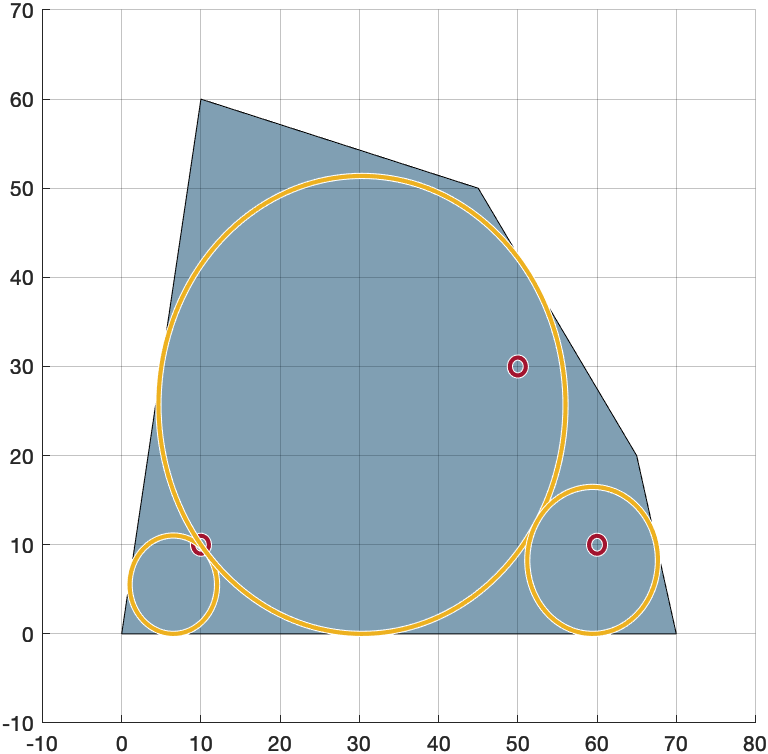
\includegraphics{hw2/prob1_plot1.png}
    \caption{Solution 1}
\end{figure}

After inspecting the plot, we think this might be a local minima. Therefore we changed the initial starting point and re-run the program and we achieved a better object value of -2388.37652.

\begin{center}
\begin{tabular}{c || c | c | c || c | c | c}
     circle & r0 & x0 & y0 & r & x & y \\
     \hline
     1     & 1  & 20 & 50 & 5.67305 & 14.5512 & 52.7669 \\
     2     & 1  & 50 & 30 & 25.6917 & 30.328 & 25.6917 \\
     3     & 1  & 60 & 10 & 8.24611 & 59.4386 & 8.24611 \\
\end{tabular}
\end{center}

We show this solution in a similar manner than the previous plot.

\begin{figure}[h]
    \centering
    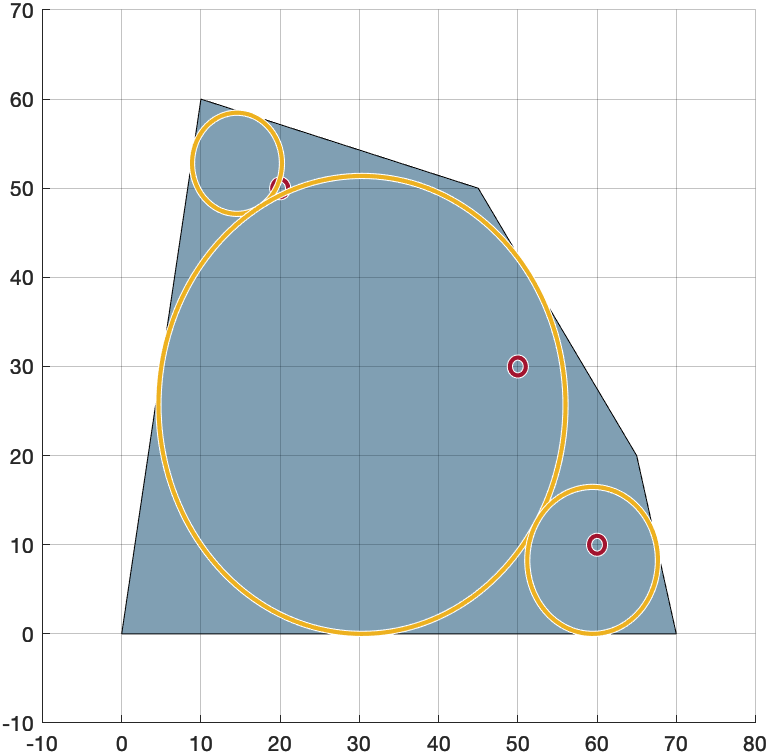
\includegraphics{hw2/prob1_plot2.png}
    \caption{Solution 2}
\end{figure}

\section{Classify Breast Cancer Patients}

Postponed till Homework 3.

\section{Stock Portfolio Investment}

Postponed till Homework 3.

\section{Solve Sunco Oil Problem with \texttt{linprog}}




\end{document}